%% The following is a directive for TeXShop to indicate the main file
%%!TEX root = diss.tex

\chapter{Methods}
\label{ch:Methods}
\section{Section}
\label{sec:section}

To carry out the integration from Eqn.~\ref{eqn:eqn1} in practice, it is necessary to have an accurate way of measuring the occupancy, $N$, of the probe dot. We measure $N$ by measuring the conductance $G_{sens}$ through a charge sensing quantum point contact (QPC) seen in Fig.~\ref{fig:device}. 
\begin{figure}[h]
\centering
\resizebox{1\textwidth}{!}{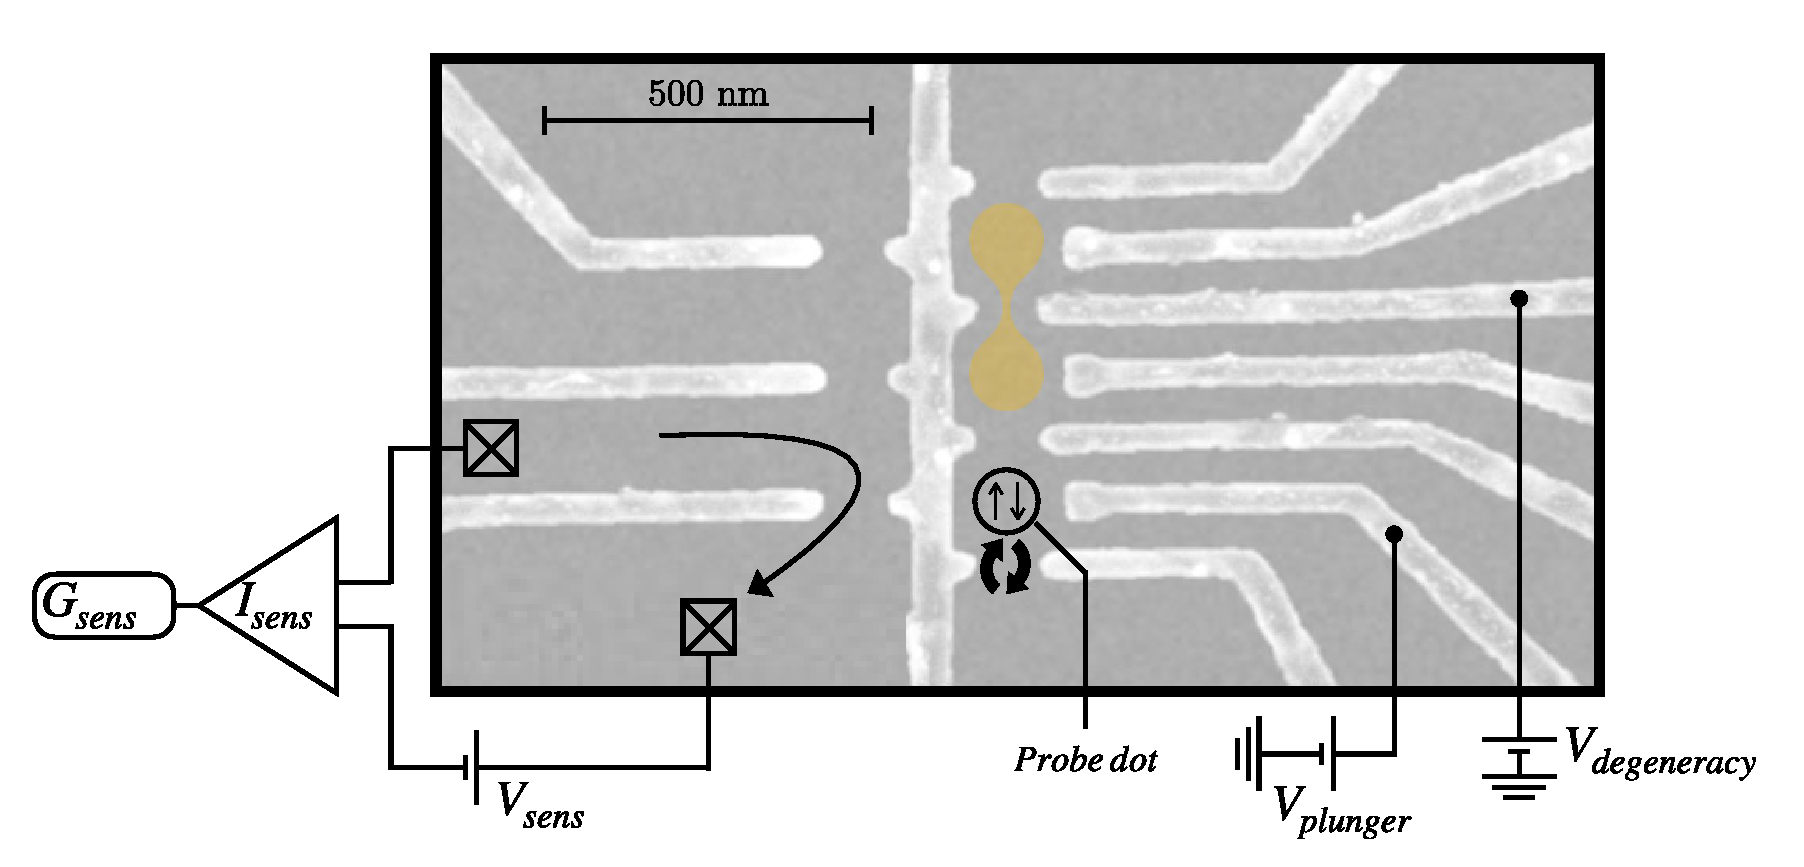
\includegraphics{figures/pdfs/device.eps}}
\caption{ A top-down SEM image of an early prototype of the proposed device. Lighter regions are the gold gates, while darker regions are the GaAs substrate. The upper pair of quantum dots highlighted in yellow will be probed by the bottommost dot whose occupation is measured using $G_{sens}$. In this prototype, temperature oscillations would occur across the substrate with electrons in the reservoir connected to the probe dot heated via coupling to the phonons of the substrate. $V_p$ will be used to control the chemical potential, $\mu$, in the probe dot. In the upper pair of dots, similar gate structures allow for the system to be tuned to be doubly degenerate. $V_d$ is used to control the degeneracy of the upper two dot system. The indicates ohmic contact to the 2DEG.}

\label{fig:device}       % Give a unique label to the figure. 
\end{figure}
Because of the proximity of this QPC, referred to as the charge sensor, to the probe dot very small electrostatic changes in the probe dot affect the conduction across the charge sensor~\cite{spintocharge}. As such, a larger $G_{sens}$ indicates fewer electrons in the probe dot, while a smaller $G_{sens}$ indicates more electrons in the probe dot. In effect, this means that $G_{sens}$ can be used to directly measure the occupancy of the dot as a function of various other quantities like chemical potential, $\mu$, or temperature, $T$. We use $V_{plunger}$ ($V_p$) shown in in Fig.~\ref{fig:device} to locally control the chemical potential of the dot. Varying the potential applied to this gate $V_p$ - and by extension the chemical potential in the dot - is our primary technique to control the occupancy of the dot. Based on this protocol, we can decompose Eqn.~\ref{eqn:eqn1} into the following quantities which can be determined experimentally.
\begin{equation}
	\label{eqn:eqn2}
	\Delta S = \int_{\mu_1}^{\mu_2} d G_{sens}\frac{dN}{dG_{sens}} \frac{1}{dT} \,\,  d \mu
\end{equation}
This integral tells us that we can measure the change in entropy between two chemical potentials in the dot by measuring three quantities: $dN/dG_{sens}$, $dT$, and $dG_{sens}$ as a function of chemical potential. The first two quantities $dN/dG_{sens}$ and $dT$ are scaling factors that can be independently experimentally determined but do not depend on $\mu$ however the final quantity $dG_{sens}$ does depend on $\mu$ and so must be measured as $\mu$ is changed. Intuitively, $dG_{sens}$ is a measure of the difference between the occupancy of the dot at higher $T$ and lower $T$ - this is illustrated by the shading on the plots in Fig.~\ref{fig:num_int}. 


\begin{figure}[h]
\centering
\resizebox{1\textwidth}{!}{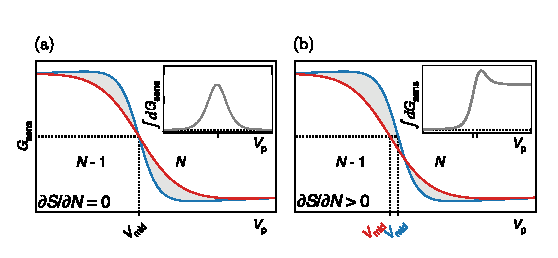
\includegraphics{figures/pdfs/numerical_integrated.eps}}
\caption{ In (a) and (b) we show two examples of the measurement protocol where the occupancy of the probe dot is measured using $G_{sens}$. In each case, the occupancy is swept from $N - 1$ to $N$ electrons both at a higher temperature (red) and a lower temperature (blue), however in (a) this change in $N$ does not correspond to an entropy change in the system whereas in (b) we see a positive change in entropy of the system due to this change in occupancy. The inlaid plots show the cumulative integral of $d G_{sens}$ -- or the difference between hot and cold $G_{sens}$ curves. The entropy change of the system is measured by the value of this integral after the completion of this transition. $V_{mid}$ is labelled for each curve, notably, $V_{mid}$ is the same in the zero entropy case, but shifts in the finite entropy case. Figure from Hartman et al.}
\label{fig:num_int}       % Give a unique label to the figure. 
\end{figure}

Using $V_{degeneracy}$ ($V_d$) the quantum system composed of the two dots (highlighted in yellow in Fig.~\ref{fig:device}) with a single electron confined within the system can be tuned between non-degenerate and doubly-degenerate. This works by first suppressing spin degrees of freedom with a large magnetic field then slowly changing the shape of the potential function separating the two dots using $V_d$. Once the potential barrier between the dots is large enough, the tunneling rate will become negligible.

Capacitive coupling between the probe dot and the pair of dots can be tuned such that occupation of the probe dot suppresses the degeneracy of the two-dot system. This is because the lowest energy state will occur when the two electrons are farthest apart. Thus, we can tune the system to a state where there is an entropy change of the entire thermodynamic system independent (while no change in entropy of the probe dot itself) as the probe dot changes occupation. In this way, we will be able to detect a non zero value of entropy if we are able to detect changes in entropy of a capacitively coupled system. Specifically, by tuning the upper two dot system between non-degenerate and doubly degenerate, we will be able to see the change as entropy as the probe dot transitions $0 \to 1$ electrons vary from $\Delta S = 0$ to $\Delta S = -\ln2$, respectively.

Preliminary evidence that we will be able to see a change in the measured entropy based on this coupling between the probe dot and another system comes from data collected on a different device coupled to an impurity in the substrate. In Fig~\ref{fig:sshape}, data from this device shows that as $V_d$ (effective) is varied, the entropy measured changes significantly. Because no parallel field is applied and the probe dot transitions from $0 \to 1$ electron, the probe dot on its own causes a change in entropy of $\Delta S/k_b = \ln 2 - \ln 1 = \ln 2 $. As such, changes in this entropy due to the impurity cause deviations in the entropy from this expected value. Clearly, this situation differs from the experiment we are proposing as there is either a positive or negative change in entropy depending on $V_d$ (effective). 

\begin{figure}[h]
\centering
\resizebox{1\textwidth}{!}{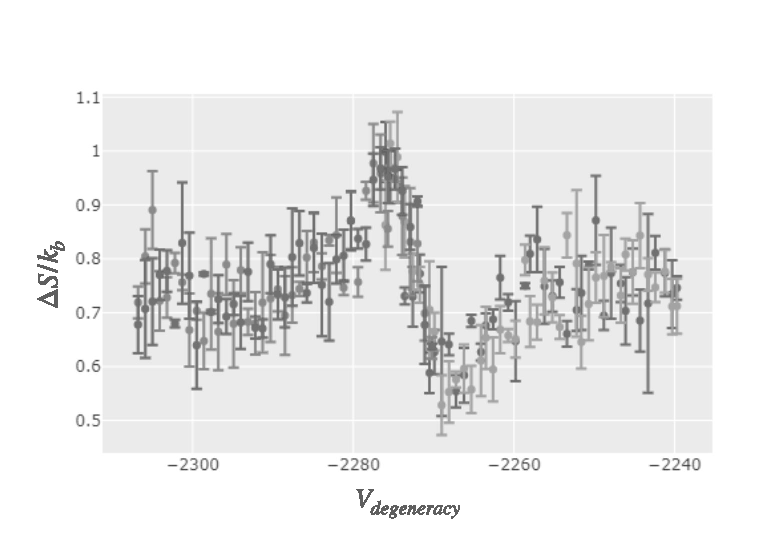
\includegraphics{figures/pdfs/temp_s_shape_bw.eps}}
\caption{ Data from an older device exhibits a change in entropy as degeneracy of an unknown external impurity is adjusted. The demonstrates the potential for measuring the entropy of capacitively coupled systems.}

\label{fig:sshape}       % Give a unique label to the figure. 
\end{figure}


The measurement protocol as laid out in Fig.~\ref{fig:num_int} requires the ability to vary the temperature of the system. However, in practice, instability in the exact locations of $V_{mid}$ makes it difficult to accurately determine $\Delta S$ of the hot and cold curves independently. Because of this instability, it is necessary to oscillate between hot and cold as we measure over the transition. With this measurement scheme, any heating not localized on the device is not useful as it will take too long to equilibrate through the entirety of whatever larger system is being heated.

We are pursuing multiple possible solutions for fast localized heating. The first is the technique employed by Hartman et al. and used in previous device designs which involves directly injecting hot electrons into the electron reservoir coupled to the probe dot. This can be done by running a current through a QPC (tuned to be fairly resistive) pointed into the electron reservoir. When the current is turned off the heat in the electron reservoir is dissipated by coupling to phonons and connection to a `cold' ground - i.e. a much larger bath of electrons at lower temperature. By turning on and off the current running through this resistive heater QPC, we can locally control the temperature of the electrons in the system. Another possible technique that could be employed to allow for fast localized heating is heating the crystalline lattice of the substrate. With this technique, the electron-phonon coupling in the electron reservoir would ensure that the electrons quickly thermalize. Resistive heating would most likely be used to heat the phonons, either by electron phonon coupling using a QPC which is electrically insulated from the device, or by building a resistor on top of the substrate using a very long wire with some finite resistance.

Devices to complete this experiment will be built on GaAs/AlGaAs heterostructure which hosts a 2DEG (see Fig \ref{fig:algaas}). The 2DEG is electrostatically gated to allow for local control of the electron density i.e. by applying an electric field with an electrically isolated gate, the electron density of the 2DEG is controlled beneath this gate \cite{Kouwenhoven1997}. Ohmic contact is made with the 2DEG via a diffusive process of Ni/Au/Ge through the substrate. Gating structures will be defined using standard photolithography and electron beam lithography techniques.  

\begin{figure}[h]
\centering
\resizebox{0.5\textwidth}{!}{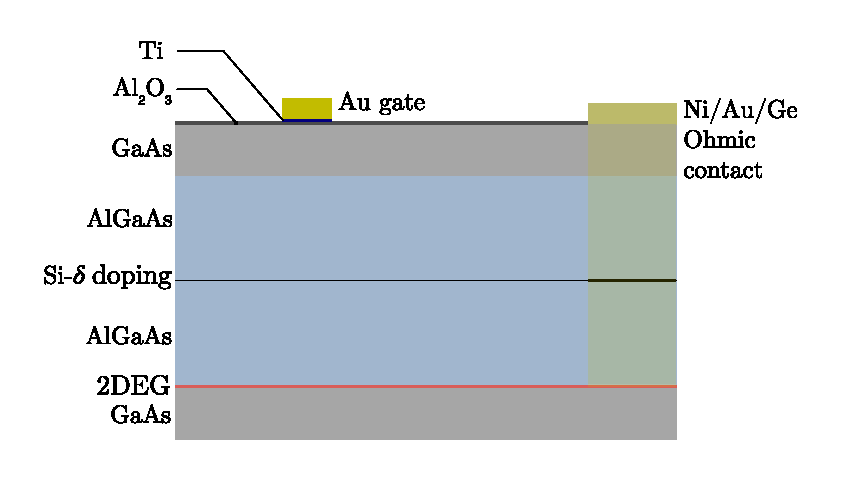
\includegraphics{figures/pdfs/algaas.eps}}
\caption{ A cross section of the GaAs/AlGaAs heterostructure hosting a 2-dimensional electron gas (2DEG) formed at the boundary between an AlGaAs and GaAs layer where the conductance band briefly falls below the Fermi energy \cite{Baer}. Gold gates allow local control of the electron density of the 2DEG. Ohmic contact to the 2DEG is established by a diffusion of a combination of Ni/Au/Ge from the surface to the 2DEG.}

\label{fig:algaas}       % Give a unique label to the figure. 
\end{figure}

\endinput

Any text after an \endinput is ignored.
You could put scraps here or things in progress.
